\documentclass[1p]{elsarticle_modified}
%\bibliographystyle{elsarticle-num}

%\usepackage[colorlinks]{hyperref}
%\usepackage{abbrmath_seonhwa} %\Abb, \Ascr, \Acal ,\Abf, \Afrak
\usepackage{amsfonts}
\usepackage{amssymb}
\usepackage{amsmath}
\usepackage{amsthm}
\usepackage{scalefnt}
\usepackage{amsbsy}
\usepackage{kotex}
\usepackage{caption}
\usepackage{subfig}
\usepackage{color}
\usepackage{graphicx}
\usepackage{xcolor} %% white, black, red, green, blue, cyan, magenta, yellow
\usepackage{float}
\usepackage{setspace}
\usepackage{hyperref}

\usepackage{tikz}
\usetikzlibrary{arrows}

\usepackage{multirow}
\usepackage{array} % fixed length table
\usepackage{hhline}

%%%%%%%%%%%%%%%%%%%%%
\makeatletter
\renewcommand*\env@matrix[1][\arraystretch]{%
	\edef\arraystretch{#1}%
	\hskip -\arraycolsep
	\let\@ifnextchar\new@ifnextchar
	\array{*\c@MaxMatrixCols c}}
\makeatother %https://tex.stackexchange.com/questions/14071/how-can-i-increase-the-line-spacing-in-a-matrix
%%%%%%%%%%%%%%%

\usepackage[normalem]{ulem}

\newcommand{\msout}[1]{\ifmmode\text{\sout{\ensuremath{#1}}}\else\sout{#1}\fi}
%SOURCE: \msout is \stkout macro in https://tex.stackexchange.com/questions/20609/strikeout-in-math-mode

\newcommand{\cancel}[1]{
	\ifmmode
	{\color{red}\msout{#1}}
	\else
	{\color{red}\sout{#1}}
	\fi
}

\newcommand{\add}[1]{
	{\color{blue}\uwave{#1}}
}

\newcommand{\replace}[2]{
	\ifmmode
	{\color{red}\msout{#1}}{\color{blue}\uwave{#2}}
	\else
	{\color{red}\sout{#1}}{\color{blue}\uwave{#2}}
	\fi
}

\newcommand{\Sol}{\mathcal{S}} %segment
\newcommand{\D}{D} %diagram
\newcommand{\A}{\mathcal{A}} %arc


%%%%%%%%%%%%%%%%%%%%%%%%%%%%%5 test

\def\sl{\operatorname{\textup{SL}}(2,\Cbb)}
\def\psl{\operatorname{\textup{PSL}}(2,\Cbb)}
\def\quan{\mkern 1mu \triangleright \mkern 1mu}

\theoremstyle{definition}
\newtheorem{thm}{Theorem}[section]
\newtheorem{prop}[thm]{Proposition}
\newtheorem{lem}[thm]{Lemma}
\newtheorem{ques}[thm]{Question}
\newtheorem{cor}[thm]{Corollary}
\newtheorem{defn}[thm]{Definition}
\newtheorem{exam}[thm]{Example}
\newtheorem{rmk}[thm]{Remark}
\newtheorem{alg}[thm]{Algorithm}

\newcommand{\I}{\sqrt{-1}}
\begin{document}

%\begin{frontmatter}
%
%\title{Boundary parabolic representations of knots up to 8 crossings}
%
%%% Group authors per affiliation:
%\author{Yunhi Cho} 
%\address{Department of Mathematics, University of Seoul, Seoul, Korea}
%\ead{yhcho@uos.ac.kr}
%
%
%\author{Seonhwa Kim} %\fnref{s_kim}}
%\address{Center for Geometry and Physics, Institute for Basic Science, Pohang, 37673, Korea}
%\ead{ryeona17@ibs.re.kr}
%
%\author{Hyuk Kim}
%\address{Department of Mathematical Sciences, Seoul National University, Seoul 08826, Korea}
%\ead{hyukkim@snu.ac.kr}
%
%\author{Seokbeom Yoon}
%\address{Department of Mathematical Sciences, Seoul National University, Seoul, 08826,  Korea}
%\ead{sbyoon15@snu.ac.kr}
%
%\begin{abstract}
%We find all boundary parabolic representation of knots up to 8 crossings.
%
%\end{abstract}
%\begin{keyword}
%    \MSC[2010] 57M25 
%\end{keyword}
%
%\end{frontmatter}

%\linenumbers
%\tableofcontents
%
\newcommand\colored[1]{\textcolor{white}{\rule[-0.35ex]{0.8em}{1.4ex}}\kern-0.8em\color{red} #1}%
%\newcommand\colored[1]{\textcolor{white}{ #1}\kern-2.17ex	\textcolor{white}{ #1}\kern-1.81ex	\textcolor{white}{ #1}\kern-2.15ex\color{red}#1	}

{\Large $\underline{11a_{130}~(K11a_{130})}$}

\setlength{\tabcolsep}{10pt}
\renewcommand{\arraystretch}{1.6}
\vspace{1cm}\begin{tabular}{m{100pt}>{\centering\arraybackslash}m{274pt}}
\multirow{5}{120pt}{
	\centering
	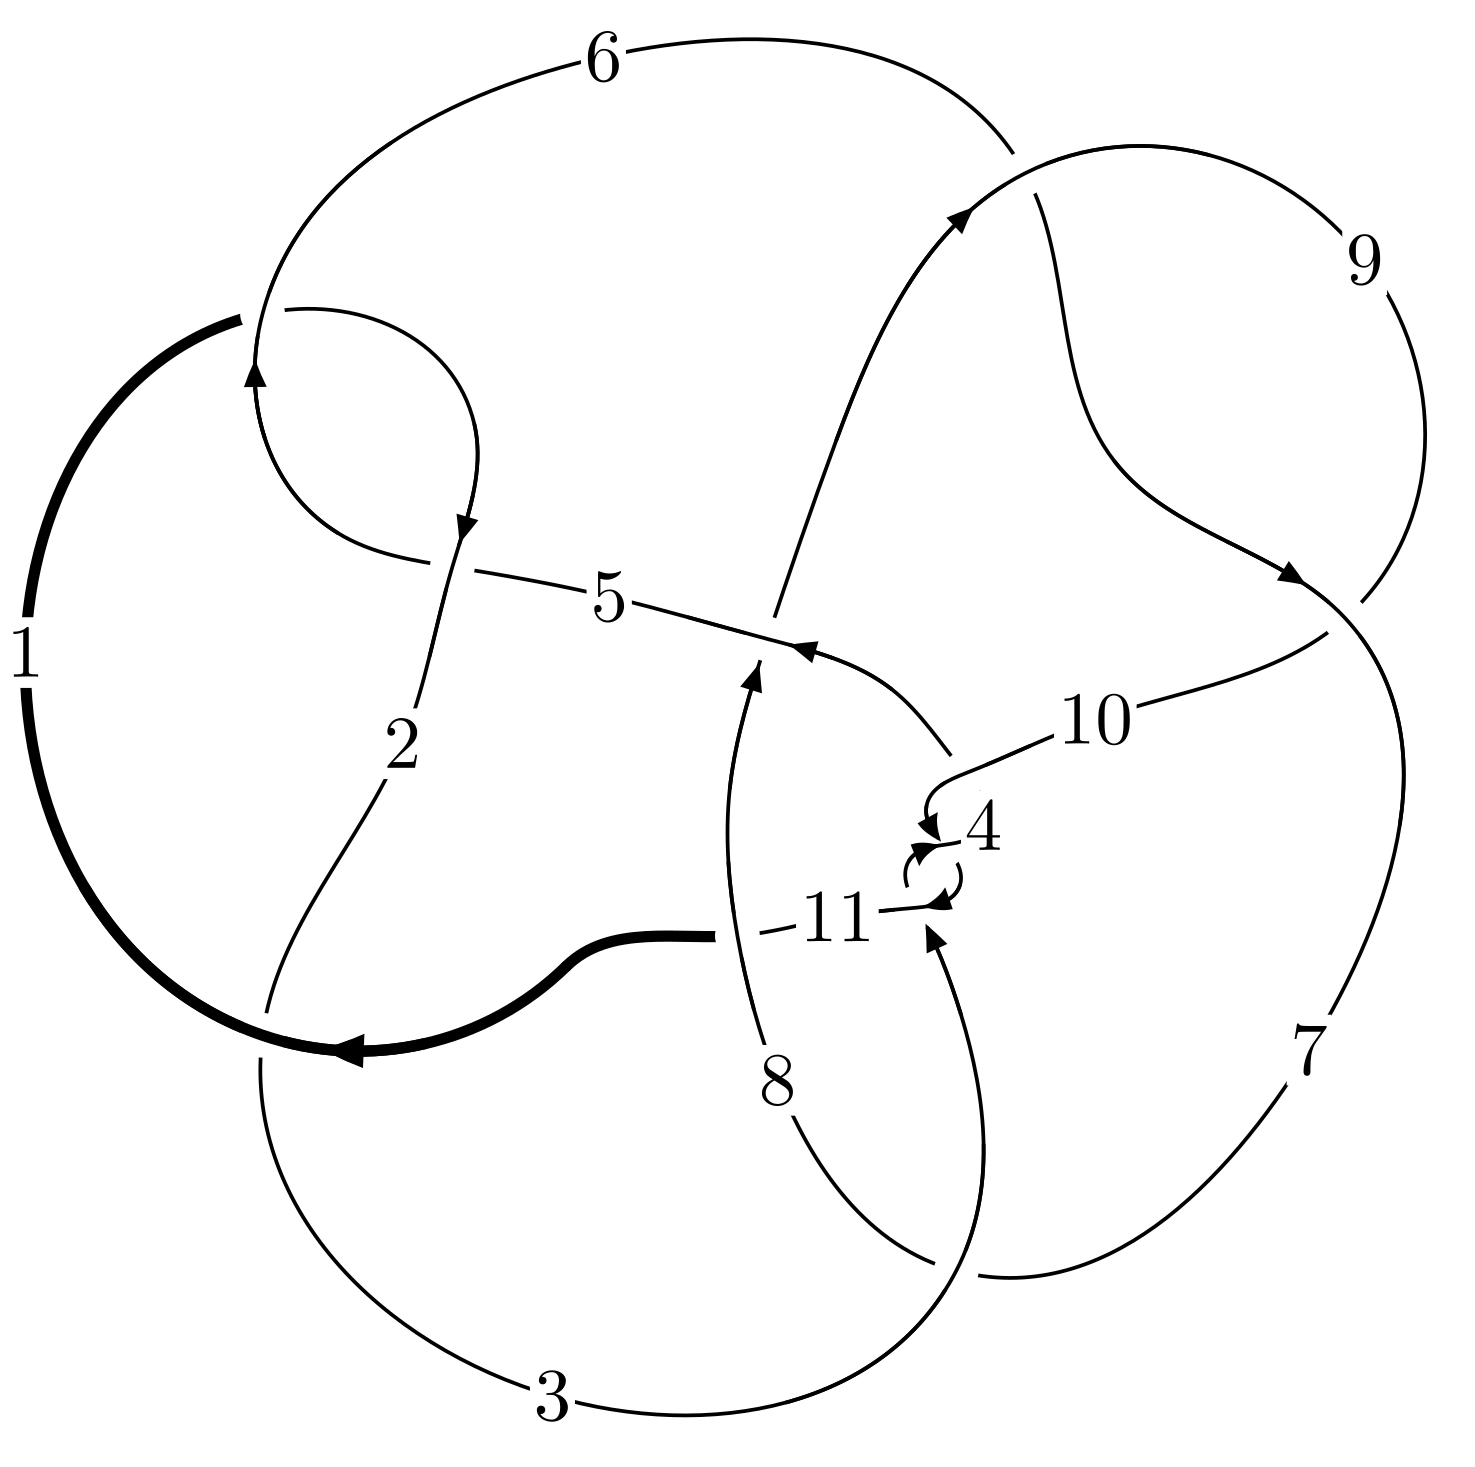
\includegraphics[width=112pt]{../../../GIT/diagram.site/Diagrams/png/379_11a_130.png}\\
\ \ \ A knot diagram\footnotemark}&
\allowdisplaybreaks
\textbf{Linearized knot diagam} \\
\cline{2-2}
 &
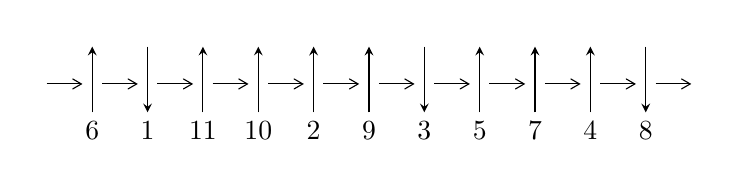
\begin{tikzpicture}[x=20pt, y=17pt]
	% nodes
	\node (C0) at (0, 0) {};
	\node (C1) at (1, 0) {};
	\node (C1U) at (1, +1) {};
	\node (C1D) at (1, -1) {6};

	\node (C2) at (2, 0) {};
	\node (C2U) at (2, +1) {};
	\node (C2D) at (2, -1) {1};

	\node (C3) at (3, 0) {};
	\node (C3U) at (3, +1) {};
	\node (C3D) at (3, -1) {11};

	\node (C4) at (4, 0) {};
	\node (C4U) at (4, +1) {};
	\node (C4D) at (4, -1) {10};

	\node (C5) at (5, 0) {};
	\node (C5U) at (5, +1) {};
	\node (C5D) at (5, -1) {2};

	\node (C6) at (6, 0) {};
	\node (C6U) at (6, +1) {};
	\node (C6D) at (6, -1) {9};

	\node (C7) at (7, 0) {};
	\node (C7U) at (7, +1) {};
	\node (C7D) at (7, -1) {3};

	\node (C8) at (8, 0) {};
	\node (C8U) at (8, +1) {};
	\node (C8D) at (8, -1) {5};

	\node (C9) at (9, 0) {};
	\node (C9U) at (9, +1) {};
	\node (C9D) at (9, -1) {7};

	\node (C10) at (10, 0) {};
	\node (C10U) at (10, +1) {};
	\node (C10D) at (10, -1) {4};

	\node (C11) at (11, 0) {};
	\node (C11U) at (11, +1) {};
	\node (C11D) at (11, -1) {8};
	\node (C12) at (12, 0) {};

	% arrows
	\draw[->,>={angle 60}]
	(C0) edge (C1) (C1) edge (C2) (C2) edge (C3) (C3) edge (C4) (C4) edge (C5) (C5) edge (C6) (C6) edge (C7) (C7) edge (C8) (C8) edge (C9) (C9) edge (C10) (C10) edge (C11) (C11) edge (C12) ;	\draw[->,>=stealth]
	(C1D) edge (C1U) (C2U) edge (C2D) (C3D) edge (C3U) (C4D) edge (C4U) (C5D) edge (C5U) (C6D) edge (C6U) (C7U) edge (C7D) (C8D) edge (C8U) (C9D) edge (C9U) (C10D) edge (C10U) (C11U) edge (C11D) ;
	\end{tikzpicture} \\
\hhline{~~} \\& 
\textbf{Solving Sequence} \\ \cline{2-2} 
 &
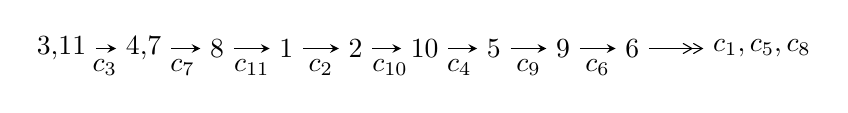
\begin{tikzpicture}[x=25pt, y=7pt]
	% node
	\node (A0) at (-1/8, 0) {3,11};
	\node (A1) at (17/16, 0) {4,7};
	\node (A2) at (17/8, 0) {8};
	\node (A3) at (25/8, 0) {1};
	\node (A4) at (33/8, 0) {2};
	\node (A5) at (41/8, 0) {10};
	\node (A6) at (49/8, 0) {5};
	\node (A7) at (57/8, 0) {9};
	\node (A8) at (65/8, 0) {6};
	\node (C1) at (1/2, -1) {$c_{3}$};
	\node (C2) at (13/8, -1) {$c_{7}$};
	\node (C3) at (21/8, -1) {$c_{11}$};
	\node (C4) at (29/8, -1) {$c_{2}$};
	\node (C5) at (37/8, -1) {$c_{10}$};
	\node (C6) at (45/8, -1) {$c_{4}$};
	\node (C7) at (53/8, -1) {$c_{9}$};
	\node (C8) at (61/8, -1) {$c_{6}$};
	\node (A9) at (10, 0) {$c_{1},c_{5},c_{8}$};

	% edge
	\draw[->,>=stealth]	
	(A0) edge (A1) (A1) edge (A2) (A2) edge (A3) (A3) edge (A4) (A4) edge (A5) (A5) edge (A6) (A6) edge (A7) (A7) edge (A8) ;
	\draw[->>,>={angle 60}]	
	(A8) edge (A9);
\end{tikzpicture} \\ 

\end{tabular} \\

\footnotetext{
The image of knot diagram is generated by the software ``\textbf{Draw programme}" developed by Andrew Bartholomew(\url{http://www.layer8.co.uk/maths/draw/index.htm\#Running-draw}), where we modified some parts for our purpose(\url{https://github.com/CATsTAILs/LinksPainter}).
}\phantom \\ \newline 
\centering \textbf{Ideals for irreducible components\footnotemark of $X_{\text{par}}$} 
 
\begin{align*}
I^u_{1}&=\langle 
1.08589\times10^{65} u^{61}-2.14541\times10^{65} u^{60}+\cdots+1.37317\times10^{65} b+1.63028\times10^{65},\\
\phantom{I^u_{1}}&\phantom{= \langle  }1.15709\times10^{65} u^{61}-2.34918\times10^{65} u^{60}+\cdots+1.37317\times10^{65} a+1.55380\times10^{65},\;u^{62}-2 u^{61}+\cdots+2 u-1\rangle \\
I^u_{2}&=\langle 
3 b+1,\;3 a+1,\;u-1\rangle \\
\\
\end{align*}
\raggedright * 2 irreducible components of $\dim_{\mathbb{C}}=0$, with total 63 representations.\\
\footnotetext{All coefficients of polynomials are rational numbers. But the coefficients are sometimes approximated in decimal forms when there is not enough margin.}
\newpage
\renewcommand{\arraystretch}{1}
\centering \section*{I. $I^u_{1}= \langle 1.09\times10^{65} u^{61}-2.15\times10^{65} u^{60}+\cdots+1.37\times10^{65} b+1.63\times10^{65},\;1.16\times10^{65} u^{61}-2.35\times10^{65} u^{60}+\cdots+1.37\times10^{65} a+1.55\times10^{65},\;u^{62}-2 u^{61}+\cdots+2 u-1 \rangle$}
\flushleft \textbf{(i) Arc colorings}\\
\begin{tabular}{m{7pt} m{180pt} m{7pt} m{180pt} }
\flushright $a_{3}=$&$\begin{pmatrix}1\\0\end{pmatrix}$ \\
\flushright $a_{11}=$&$\begin{pmatrix}0\\u\end{pmatrix}$ \\
\flushright $a_{4}=$&$\begin{pmatrix}1\\- u^2\end{pmatrix}$ \\
\flushright $a_{7}=$&$\begin{pmatrix}-0.842640 u^{61}+1.71077 u^{60}+\cdots-2.66212 u-1.13154\\-0.790788 u^{61}+1.56238 u^{60}+\cdots+2.05964 u-1.18724\end{pmatrix}$ \\
\flushright $a_{8}=$&$\begin{pmatrix}-0.0518518 u^{61}+0.148389 u^{60}+\cdots-4.72176 u+0.0556948\\-0.790788 u^{61}+1.56238 u^{60}+\cdots+2.05964 u-1.18724\end{pmatrix}$ \\
\flushright $a_{1}=$&$\begin{pmatrix}0.341402 u^{61}-0.580498 u^{60}+\cdots-0.691103 u+0.320601\\-0.235284 u^{61}+0.469850 u^{60}+\cdots-1.26969 u-0.112987\end{pmatrix}$ \\
\flushright $a_{2}=$&$\begin{pmatrix}0.252650 u^{61}-0.150172 u^{60}+\cdots+0.0795973 u+1.03377\\-0.109160 u^{61}-0.0358719 u^{60}+\cdots-0.212253 u+0.116597\end{pmatrix}$ \\
\flushright $a_{10}=$&$\begin{pmatrix}- u\\u^3+u\end{pmatrix}$ \\
\flushright $a_{5}=$&$\begin{pmatrix}u^2+1\\- u^4-2 u^2\end{pmatrix}$ \\
\flushright $a_{9}=$&$\begin{pmatrix}-0.792952 u^{61}+1.65665 u^{60}+\cdots-4.07865 u-1.02885\\-0.744507 u^{61}+1.47164 u^{60}+\cdots+3.24890 u-1.22506\end{pmatrix}$ \\
\flushright $a_{6}=$&$\begin{pmatrix}-0.183781 u^{61}+0.268627 u^{60}+\cdots+1.82401 u-0.309920\\-0.100621 u^{61}+0.180677 u^{60}+\cdots-1.14699 u+0.0882537\end{pmatrix}$\\ \flushright $a_{6}=$&$\begin{pmatrix}-0.183781 u^{61}+0.268627 u^{60}+\cdots+1.82401 u-0.309920\\-0.100621 u^{61}+0.180677 u^{60}+\cdots-1.14699 u+0.0882537\end{pmatrix}$\\&\end{tabular}
\flushleft \textbf{(ii) Obstruction class $= -1$}\\~\\
\flushleft \textbf{(iii) Cusp Shapes $= -1.87855 u^{61}+4.80262 u^{60}+\cdots+9.92096 u-3.84759$}\\~\\
\newpage\renewcommand{\arraystretch}{1}
\flushleft \textbf{(iv) u-Polynomials at the component}\newline \\
\begin{tabular}{m{50pt}|m{274pt}}
Crossings & \hspace{64pt}u-Polynomials at each crossing \\
\hline $$\begin{aligned}c_{1},c_{5}\end{aligned}$$&$\begin{aligned}
&u^{62}-2 u^{61}+\cdots-2 u+1
\end{aligned}$\\
\hline $$\begin{aligned}c_{2}\end{aligned}$$&$\begin{aligned}
&u^{62}+22 u^{61}+\cdots-8 u+1
\end{aligned}$\\
\hline $$\begin{aligned}c_{3},c_{4},c_{10}\end{aligned}$$&$\begin{aligned}
&u^{62}+2 u^{61}+\cdots-2 u-1
\end{aligned}$\\
\hline $$\begin{aligned}c_{6},c_{9}\end{aligned}$$&$\begin{aligned}
&u^{62}+2 u^{61}+\cdots-4 u-9
\end{aligned}$\\
\hline $$\begin{aligned}c_{7}\end{aligned}$$&$\begin{aligned}
&3(3 u^{62}-52 u^{61}+\cdots+308 u+49)
\end{aligned}$\\
\hline $$\begin{aligned}c_{8}\end{aligned}$$&$\begin{aligned}
&3(3 u^{62}+43 u^{61}+\cdots+708 u-62)
\end{aligned}$\\
\hline $$\begin{aligned}c_{11}\end{aligned}$$&$\begin{aligned}
&u^{62}+5 u^{61}+\cdots+36 u+18
\end{aligned}$\\
\hline
\end{tabular}\\~\\
\newpage\renewcommand{\arraystretch}{1}
\flushleft \textbf{(v) Riley Polynomials at the component}\newline \\
\begin{tabular}{m{50pt}|m{274pt}}
Crossings & \hspace{64pt}Riley Polynomials at each crossing \\
\hline $$\begin{aligned}c_{1},c_{5}\end{aligned}$$&$\begin{aligned}
&y^{62}+22 y^{61}+\cdots-8 y+1
\end{aligned}$\\
\hline $$\begin{aligned}c_{2}\end{aligned}$$&$\begin{aligned}
&y^{62}+30 y^{61}+\cdots-352 y+1
\end{aligned}$\\
\hline $$\begin{aligned}c_{3},c_{4},c_{10}\end{aligned}$$&$\begin{aligned}
&y^{62}+58 y^{61}+\cdots-8 y+1
\end{aligned}$\\
\hline $$\begin{aligned}c_{6},c_{9}\end{aligned}$$&$\begin{aligned}
&y^{62}-38 y^{61}+\cdots+524 y+81
\end{aligned}$\\
\hline $$\begin{aligned}c_{7}\end{aligned}$$&$\begin{aligned}
&9(9 y^{62}-1042 y^{61}+\cdots-72128 y+2401)
\end{aligned}$\\
\hline $$\begin{aligned}c_{8}\end{aligned}$$&$\begin{aligned}
&9(9 y^{62}-1081 y^{61}+\cdots+151348 y+3844)
\end{aligned}$\\
\hline $$\begin{aligned}c_{11}\end{aligned}$$&$\begin{aligned}
&y^{62}-9 y^{61}+\cdots-180 y+324
\end{aligned}$\\
\hline
\end{tabular}\\~\\
\newpage\flushleft \textbf{(vi) Complex Volumes and Cusp Shapes}
$$\begin{array}{c|c|c}  
\text{Solutions to }I^u_{1}& \I (\text{vol} + \sqrt{-1}CS) & \text{Cusp shape}\\
 \hline 
\begin{aligned}
u &= -0.854708 + 0.475494 I \\
a &= -0.501387 + 0.218656 I \\
b &= -0.766880 - 1.014110 I\end{aligned}
 & \phantom{-}5.21542 - 5.84748 I & \phantom{-0.000000 -}0. + 5.18141 I \\ \hline\begin{aligned}
u &= -0.854708 - 0.475494 I \\
a &= -0.501387 - 0.218656 I \\
b &= -0.766880 + 1.014110 I\end{aligned}
 & \phantom{-}5.21542 + 5.84748 I & \phantom{-0.000000 } 0. - 5.18141 I \\ \hline\begin{aligned}
u &= \phantom{-}0.786648 + 0.683133 I \\
a &= \phantom{-}0.435125 - 0.646494 I \\
b &= -0.564398 - 0.724669 I\end{aligned}
 & \phantom{-}3.00308 - 6.49550 I & \phantom{-0.000000 } 0 \\ \hline\begin{aligned}
u &= \phantom{-}0.786648 - 0.683133 I \\
a &= \phantom{-}0.435125 + 0.646494 I \\
b &= -0.564398 + 0.724669 I\end{aligned}
 & \phantom{-}3.00308 + 6.49550 I & \phantom{-0.000000 } 0 \\ \hline\begin{aligned}
u &= \phantom{-}0.828519 + 0.476769 I \\
a &= \phantom{-}0.527967 + 0.318651 I \\
b &= \phantom{-}0.93975 - 1.10440 I\end{aligned}
 & \phantom{-}3.57519 + 11.87880 I & \phantom{-}5.00000 - 8.97401 I \\ \hline\begin{aligned}
u &= \phantom{-}0.828519 - 0.476769 I \\
a &= \phantom{-}0.527967 - 0.318651 I \\
b &= \phantom{-}0.93975 + 1.10440 I\end{aligned}
 & \phantom{-}3.57519 - 11.87880 I & \phantom{-}5.00000 + 8.97401 I \\ \hline\begin{aligned}
u &= \phantom{-}0.834218 + 0.349760 I \\
a &= \phantom{-}0.205591 + 0.243605 I \\
b &= \phantom{-}0.939722 - 0.468213 I\end{aligned}
 & -2.11951 + 4.18883 I & \phantom{-}1.15636 - 7.37516 I \\ \hline\begin{aligned}
u &= \phantom{-}0.834218 - 0.349760 I \\
a &= \phantom{-}0.205591 - 0.243605 I \\
b &= \phantom{-}0.939722 + 0.468213 I\end{aligned}
 & -2.11951 - 4.18883 I & \phantom{-}1.15636 + 7.37516 I \\ \hline\begin{aligned}
u &= -0.858558 + 0.732202 I \\
a &= -0.324943 - 0.468199 I \\
b &= \phantom{-}0.329628 - 0.628618 I\end{aligned}
 & \phantom{-}4.56334 + 0.20821 I & \phantom{-0.000000 } 0 \\ \hline\begin{aligned}
u &= -0.858558 - 0.732202 I \\
a &= -0.324943 + 0.468199 I \\
b &= \phantom{-}0.329628 + 0.628618 I\end{aligned}
 & \phantom{-}4.56334 - 0.20821 I & \phantom{-0.000000 } 0\\
 \hline 
 \end{array}$$\newpage$$\begin{array}{c|c|c}  
\text{Solutions to }I^u_{1}& \I (\text{vol} + \sqrt{-1}CS) & \text{Cusp shape}\\
 \hline 
\begin{aligned}
u &= -1.19372\phantom{ +0.000000I} \\
a &= -0.137031\phantom{ +0.000000I} \\
b &= -0.442772\phantom{ +0.000000I}\end{aligned}
 & \phantom{-}3.07751\phantom{ +0.000000I} & \phantom{-0.000000 } 0 \\ \hline\begin{aligned}
u &= \phantom{-}0.489192 + 0.594790 I \\
a &= -0.182908 - 1.042450 I \\
b &= -0.692845 + 0.109180 I\end{aligned}
 & -3.46490 + 0.19843 I & -2.36990 - 1.02428 I \\ \hline\begin{aligned}
u &= \phantom{-}0.489192 - 0.594790 I \\
a &= -0.182908 + 1.042450 I \\
b &= -0.692845 - 0.109180 I\end{aligned}
 & -3.46490 - 0.19843 I & -2.36990 + 1.02428 I \\ \hline\begin{aligned}
u &= \phantom{-}0.017185 + 1.247160 I \\
a &= \phantom{-}0.162682 - 0.287701 I \\
b &= -0.013266 + 1.237940 I\end{aligned}
 & \phantom{-}1.05860 + 2.54967 I & \phantom{-0.000000 } 0 \\ \hline\begin{aligned}
u &= \phantom{-}0.017185 - 1.247160 I \\
a &= \phantom{-}0.162682 + 0.287701 I \\
b &= -0.013266 - 1.237940 I\end{aligned}
 & \phantom{-}1.05860 - 2.54967 I & \phantom{-0.000000 } 0 \\ \hline\begin{aligned}
u &= \phantom{-}0.537923 + 0.421196 I \\
a &= -0.66395 - 1.42924 I \\
b &= -0.874587 + 0.713367 I\end{aligned}
 & -0.54466 + 6.46296 I & \phantom{-}3.86014 - 8.94603 I \\ \hline\begin{aligned}
u &= \phantom{-}0.537923 - 0.421196 I \\
a &= -0.66395 + 1.42924 I \\
b &= -0.874587 - 0.713367 I\end{aligned}
 & -0.54466 - 6.46296 I & \phantom{-}3.86014 + 8.94603 I \\ \hline\begin{aligned}
u &= \phantom{-}0.126822 + 1.321270 I \\
a &= \phantom{-}1.46059 - 0.50935 I \\
b &= \phantom{-}0.169563 + 0.083121 I\end{aligned}
 & -0.24430 + 1.55160 I & \phantom{-0.000000 } 0 \\ \hline\begin{aligned}
u &= \phantom{-}0.126822 - 1.321270 I \\
a &= \phantom{-}1.46059 + 0.50935 I \\
b &= \phantom{-}0.169563 - 0.083121 I\end{aligned}
 & -0.24430 - 1.55160 I & \phantom{-0.000000 } 0 \\ \hline\begin{aligned}
u &= -0.146235 + 1.336670 I \\
a &= -1.61705 - 0.58737 I \\
b &= -0.154694 - 0.262432 I\end{aligned}
 & -0.85413 - 6.64291 I & \phantom{-0.000000 } 0\\
 \hline 
 \end{array}$$\newpage$$\begin{array}{c|c|c}  
\text{Solutions to }I^u_{1}& \I (\text{vol} + \sqrt{-1}CS) & \text{Cusp shape}\\
 \hline 
\begin{aligned}
u &= -0.146235 - 1.336670 I \\
a &= -1.61705 + 0.58737 I \\
b &= -0.154694 + 0.262432 I\end{aligned}
 & -0.85413 + 6.64291 I & \phantom{-0.000000 } 0 \\ \hline\begin{aligned}
u &= \phantom{-}0.056128 + 1.345530 I \\
a &= \phantom{-}1.61787 + 0.49934 I \\
b &= \phantom{-}1.11617 + 1.02320 I\end{aligned}
 & -2.08593 + 1.24865 I & \phantom{-0.000000 } 0 \\ \hline\begin{aligned}
u &= \phantom{-}0.056128 - 1.345530 I \\
a &= \phantom{-}1.61787 - 0.49934 I \\
b &= \phantom{-}1.11617 - 1.02320 I\end{aligned}
 & -2.08593 - 1.24865 I & \phantom{-0.000000 } 0 \\ \hline\begin{aligned}
u &= -0.479881 + 0.382241 I \\
a &= \phantom{-}0.86897 - 1.13609 I \\
b &= \phantom{-}0.593189 + 0.758731 I\end{aligned}
 & \phantom{-}0.78887 - 1.60795 I & \phantom{-}6.50613 + 4.85102 I \\ \hline\begin{aligned}
u &= -0.479881 - 0.382241 I \\
a &= \phantom{-}0.86897 + 1.13609 I \\
b &= \phantom{-}0.593189 - 0.758731 I\end{aligned}
 & \phantom{-}0.78887 + 1.60795 I & \phantom{-}6.50613 - 4.85102 I \\ \hline\begin{aligned}
u &= -0.024388 + 1.403660 I \\
a &= -8.25761 + 1.43088 I \\
b &= -8.06787 + 1.51488 I\end{aligned}
 & -3.33744 + 1.94948 I & \phantom{-0.000000 } 0 \\ \hline\begin{aligned}
u &= -0.024388 - 1.403660 I \\
a &= -8.25761 - 1.43088 I \\
b &= -8.06787 - 1.51488 I\end{aligned}
 & -3.33744 - 1.94948 I & \phantom{-0.000000 } 0 \\ \hline\begin{aligned}
u &= -0.099048 + 1.403400 I \\
a &= -1.84560 - 0.69536 I \\
b &= -1.172890 - 0.762039 I\end{aligned}
 & -4.73418 - 2.70185 I & \phantom{-0.000000 } 0 \\ \hline\begin{aligned}
u &= -0.099048 - 1.403400 I \\
a &= -1.84560 + 0.69536 I \\
b &= -1.172890 + 0.762039 I\end{aligned}
 & -4.73418 + 2.70185 I & \phantom{-0.000000 } 0 \\ \hline\begin{aligned}
u &= \phantom{-}0.356454 + 1.365780 I \\
a &= -0.896048 - 0.640586 I \\
b &= -0.915691 - 0.086245 I\end{aligned}
 & -4.97349 - 0.07836 I & \phantom{-0.000000 } 0\\
 \hline 
 \end{array}$$\newpage$$\begin{array}{c|c|c}  
\text{Solutions to }I^u_{1}& \I (\text{vol} + \sqrt{-1}CS) & \text{Cusp shape}\\
 \hline 
\begin{aligned}
u &= \phantom{-}0.356454 - 1.365780 I \\
a &= -0.896048 + 0.640586 I \\
b &= -0.915691 + 0.086245 I\end{aligned}
 & -4.97349 + 0.07836 I & \phantom{-0.000000 } 0 \\ \hline\begin{aligned}
u &= \phantom{-}0.484112 + 0.293337 I \\
a &= -0.371899 + 0.237707 I \\
b &= \phantom{-}0.942298 + 0.544052 I\end{aligned}
 & -0.34287 - 3.16265 I & \phantom{-}3.47830 + 1.04615 I \\ \hline\begin{aligned}
u &= \phantom{-}0.484112 - 0.293337 I \\
a &= -0.371899 - 0.237707 I \\
b &= \phantom{-}0.942298 - 0.544052 I\end{aligned}
 & -0.34287 + 3.16265 I & \phantom{-}3.47830 - 1.04615 I \\ \hline\begin{aligned}
u &= -0.516231 + 0.142983 I \\
a &= \phantom{-}2.34094 - 0.73876 I \\
b &= -0.092583 + 0.868567 I\end{aligned}
 & \phantom{-}3.74985 - 4.26844 I & \phantom{-}11.92903 + 7.28144 I \\ \hline\begin{aligned}
u &= -0.516231 - 0.142983 I \\
a &= \phantom{-}2.34094 + 0.73876 I \\
b &= -0.092583 - 0.868567 I\end{aligned}
 & \phantom{-}3.74985 + 4.26844 I & \phantom{-}11.92903 - 7.28144 I \\ \hline\begin{aligned}
u &= -0.17339 + 1.45631 I \\
a &= -1.57036 - 0.03554 I \\
b &= -0.906111 - 0.957483 I\end{aligned}
 & -5.19208 - 4.01888 I & \phantom{-0.000000 } 0 \\ \hline\begin{aligned}
u &= -0.17339 - 1.45631 I \\
a &= -1.57036 + 0.03554 I \\
b &= -0.906111 + 0.957483 I\end{aligned}
 & -5.19208 + 4.01888 I & \phantom{-0.000000 } 0 \\ \hline\begin{aligned}
u &= -0.07310 + 1.46676 I \\
a &= -0.785313 - 0.776260 I \\
b &= -0.523873 - 1.073670 I\end{aligned}
 & -4.86855 - 2.39184 I & \phantom{-0.000000 } 0 \\ \hline\begin{aligned}
u &= -0.07310 - 1.46676 I \\
a &= -0.785313 + 0.776260 I \\
b &= -0.523873 + 1.073670 I\end{aligned}
 & -4.86855 + 2.39184 I & \phantom{-0.000000 } 0 \\ \hline\begin{aligned}
u &= \phantom{-}0.19203 + 1.46284 I \\
a &= \phantom{-}1.65883 + 0.15373 I \\
b &= \phantom{-}1.03342 - 1.00736 I\end{aligned}
 & -6.64439 + 9.14751 I & \phantom{-0.000000 } 0\\
 \hline 
 \end{array}$$\newpage$$\begin{array}{c|c|c}  
\text{Solutions to }I^u_{1}& \I (\text{vol} + \sqrt{-1}CS) & \text{Cusp shape}\\
 \hline 
\begin{aligned}
u &= \phantom{-}0.19203 - 1.46284 I \\
a &= \phantom{-}1.65883 - 0.15373 I \\
b &= \phantom{-}1.03342 + 1.00736 I\end{aligned}
 & -6.64439 - 9.14751 I & \phantom{-0.000000 } 0 \\ \hline\begin{aligned}
u &= \phantom{-}0.506831 + 0.096686 I \\
a &= -2.48548 - 0.48498 I \\
b &= \phantom{-}0.165777 + 0.615510 I\end{aligned}
 & \phantom{-}4.11698 - 0.69808 I & \phantom{-}13.39590 - 0.06993 I \\ \hline\begin{aligned}
u &= \phantom{-}0.506831 - 0.096686 I \\
a &= -2.48548 + 0.48498 I \\
b &= \phantom{-}0.165777 - 0.615510 I\end{aligned}
 & \phantom{-}4.11698 + 0.69808 I & \phantom{-}13.39590 + 0.06993 I \\ \hline\begin{aligned}
u &= \phantom{-}0.17217 + 1.50217 I \\
a &= \phantom{-}1.180340 + 0.239805 I \\
b &= \phantom{-}0.973547 - 0.684251 I\end{aligned}
 & -10.23620 + 2.66149 I & \phantom{-0.000000 } 0 \\ \hline\begin{aligned}
u &= \phantom{-}0.17217 - 1.50217 I \\
a &= \phantom{-}1.180340 - 0.239805 I \\
b &= \phantom{-}0.973547 + 0.684251 I\end{aligned}
 & -10.23620 - 2.66149 I & \phantom{-0.000000 } 0 \\ \hline\begin{aligned}
u &= \phantom{-}0.30961 + 1.48362 I \\
a &= -1.62839 - 0.14045 I \\
b &= -1.38181 + 0.69978 I\end{aligned}
 & -8.08648 + 8.33462 I & \phantom{-0.000000 } 0 \\ \hline\begin{aligned}
u &= \phantom{-}0.30961 - 1.48362 I \\
a &= -1.62839 + 0.14045 I \\
b &= -1.38181 - 0.69978 I\end{aligned}
 & -8.08648 - 8.33462 I & \phantom{-0.000000 } 0 \\ \hline\begin{aligned}
u &= -0.37255 + 1.47837 I \\
a &= \phantom{-}1.073200 - 0.107474 I \\
b &= \phantom{-}0.847659 + 0.449176 I\end{aligned}
 & -2.26534 - 5.42283 I & \phantom{-0.000000 } 0 \\ \hline\begin{aligned}
u &= -0.37255 - 1.47837 I \\
a &= \phantom{-}1.073200 + 0.107474 I \\
b &= \phantom{-}0.847659 - 0.449176 I\end{aligned}
 & -2.26534 + 5.42283 I & \phantom{-0.000000 } 0 \\ \hline\begin{aligned}
u &= -0.345940 + 0.314360 I \\
a &= \phantom{-}0.691718 + 0.084915 I \\
b &= -0.339879 + 0.970968 I\end{aligned}
 & \phantom{-}0.771077 - 1.084410 I & \phantom{-}6.64507 + 5.83005 I\\
 \hline 
 \end{array}$$\newpage$$\begin{array}{c|c|c}  
\text{Solutions to }I^u_{1}& \I (\text{vol} + \sqrt{-1}CS) & \text{Cusp shape}\\
 \hline 
\begin{aligned}
u &= -0.345940 - 0.314360 I \\
a &= \phantom{-}0.691718 - 0.084915 I \\
b &= -0.339879 - 0.970968 I\end{aligned}
 & \phantom{-}0.771077 + 1.084410 I & \phantom{-}6.64507 - 5.83005 I \\ \hline\begin{aligned}
u &= -0.362744 + 0.281740 I \\
a &= \phantom{-}1.140060 - 0.294583 I \\
b &= \phantom{-}0.206349 + 0.912447 I\end{aligned}
 & \phantom{-}0.631390 - 1.069140 I & \phantom{-}6.33384 + 6.12642 I \\ \hline\begin{aligned}
u &= -0.362744 - 0.281740 I \\
a &= \phantom{-}1.140060 + 0.294583 I \\
b &= \phantom{-}0.206349 - 0.912447 I\end{aligned}
 & \phantom{-}0.631390 + 1.069140 I & \phantom{-}6.33384 - 6.12642 I \\ \hline\begin{aligned}
u &= \phantom{-}0.30069 + 1.51433 I \\
a &= -1.84162 + 0.31312 I \\
b &= -1.34082 + 1.27068 I\end{aligned}
 & -2.8670 + 15.9906 I & \phantom{-0.000000 } 0 \\ \hline\begin{aligned}
u &= \phantom{-}0.30069 - 1.51433 I \\
a &= -1.84162 - 0.31312 I \\
b &= -1.34082 - 1.27068 I\end{aligned}
 & -2.8670 - 15.9906 I & \phantom{-0.000000 } 0 \\ \hline\begin{aligned}
u &= -0.30976 + 1.51386 I \\
a &= \phantom{-}1.67471 + 0.29668 I \\
b &= \phantom{-}1.18463 + 1.15509 I\end{aligned}
 & -1.20729 - 10.07420 I & \phantom{-0.000000 } 0 \\ \hline\begin{aligned}
u &= -0.30976 - 1.51386 I \\
a &= \phantom{-}1.67471 - 0.29668 I \\
b &= \phantom{-}1.18463 - 1.15509 I\end{aligned}
 & -1.20729 + 10.07420 I & \phantom{-0.000000 } 0 \\ \hline\begin{aligned}
u &= -0.061045 + 0.399084 I \\
a &= \phantom{-}0.245153 + 0.689749 I \\
b &= -0.01690 + 2.26843 I\end{aligned}
 & \phantom{-}2.17222 + 2.29029 I & -6.76562 + 2.81680 I \\ \hline\begin{aligned}
u &= -0.061045 - 0.399084 I \\
a &= \phantom{-}0.245153 - 0.689749 I \\
b &= -0.01690 - 2.26843 I\end{aligned}
 & \phantom{-}2.17222 - 2.29029 I & -6.76562 - 2.81680 I \\ \hline\begin{aligned}
u &= \phantom{-}0.10761 + 1.63393 I \\
a &= \phantom{-}0.225146 + 0.198889 I \\
b &= \phantom{-}0.322471 - 0.217860 I\end{aligned}
 & -5.19332 - 2.98425 I & \phantom{-0.000000 } 0\\
 \hline 
 \end{array}$$\newpage$$\begin{array}{c|c|c}  
\text{Solutions to }I^u_{1}& \I (\text{vol} + \sqrt{-1}CS) & \text{Cusp shape}\\
 \hline 
\begin{aligned}
u &= \phantom{-}0.10761 - 1.63393 I \\
a &= \phantom{-}0.225146 - 0.198889 I \\
b &= \phantom{-}0.322471 + 0.217860 I\end{aligned}
 & -5.19332 + 2.98425 I & \phantom{-0.000000 } 0 \\ \hline\begin{aligned}
u &= \phantom{-}0.336606\phantom{ +0.000000I} \\
a &= -2.26896\phantom{ +0.000000I} \\
b &= -0.768700\phantom{ +0.000000I}\end{aligned}
 & \phantom{-}2.13260\phantom{ +0.000000I} & \phantom{-}1.50210\phantom{ +0.000000I}\\
 \hline 
 \end{array}$$\newpage\newpage\renewcommand{\arraystretch}{1}
\centering \section*{II. $I^u_{2}= \langle 3 b+1,\;3 a+1,\;u-1 \rangle$}
\flushleft \textbf{(i) Arc colorings}\\
\begin{tabular}{m{7pt} m{180pt} m{7pt} m{180pt} }
\flushright $a_{3}=$&$\begin{pmatrix}1\\0\end{pmatrix}$ \\
\flushright $a_{11}=$&$\begin{pmatrix}0\\1\end{pmatrix}$ \\
\flushright $a_{4}=$&$\begin{pmatrix}1\\-1\end{pmatrix}$ \\
\flushright $a_{7}=$&$\begin{pmatrix}-0.333333\\-0.333333\end{pmatrix}$ \\
\flushright $a_{8}=$&$\begin{pmatrix}0\\-0.333333\end{pmatrix}$ \\
\flushright $a_{1}=$&$\begin{pmatrix}0\\1\end{pmatrix}$ \\
\flushright $a_{2}=$&$\begin{pmatrix}1\\-1\end{pmatrix}$ \\
\flushright $a_{10}=$&$\begin{pmatrix}-1\\2\end{pmatrix}$ \\
\flushright $a_{5}=$&$\begin{pmatrix}2\\-3\end{pmatrix}$ \\
\flushright $a_{9}=$&$\begin{pmatrix}-1.33333\\1.66667\end{pmatrix}$ \\
\flushright $a_{6}=$&$\begin{pmatrix}1\\-2\end{pmatrix}$\\ \flushright $a_{6}=$&$\begin{pmatrix}1\\-2\end{pmatrix}$\\&\end{tabular}
\flushleft \textbf{(ii) Obstruction class $= 1$}\\~\\
\flushleft \textbf{(iii) Cusp Shapes $= 19.1111$}\\~\\
\newpage\renewcommand{\arraystretch}{1}
\flushleft \textbf{(iv) u-Polynomials at the component}\newline \\
\begin{tabular}{m{50pt}|m{274pt}}
Crossings & \hspace{64pt}u-Polynomials at each crossing \\
\hline $$\begin{aligned}c_{1},c_{6},c_{10}\end{aligned}$$&$\begin{aligned}
&u+1
\end{aligned}$\\
\hline $$\begin{aligned}c_{2},c_{3},c_{4}\\c_{5},c_{9}\end{aligned}$$&$\begin{aligned}
&u-1
\end{aligned}$\\
\hline $$\begin{aligned}c_{7}\end{aligned}$$&$\begin{aligned}
&3(3 u-1)
\end{aligned}$\\
\hline $$\begin{aligned}c_{8}\end{aligned}$$&$\begin{aligned}
&3(3 u-2)
\end{aligned}$\\
\hline $$\begin{aligned}c_{11}\end{aligned}$$&$\begin{aligned}
&u
\end{aligned}$\\
\hline
\end{tabular}\\~\\
\newpage\renewcommand{\arraystretch}{1}
\flushleft \textbf{(v) Riley Polynomials at the component}\newline \\
\begin{tabular}{m{50pt}|m{274pt}}
Crossings & \hspace{64pt}Riley Polynomials at each crossing \\
\hline $$\begin{aligned}c_{1},c_{2},c_{3}\\c_{4},c_{5},c_{6}\\c_{9},c_{10}\end{aligned}$$&$\begin{aligned}
&y-1
\end{aligned}$\\
\hline $$\begin{aligned}c_{7}\end{aligned}$$&$\begin{aligned}
&9(9 y-1)
\end{aligned}$\\
\hline $$\begin{aligned}c_{8}\end{aligned}$$&$\begin{aligned}
&9(9 y-4)
\end{aligned}$\\
\hline $$\begin{aligned}c_{11}\end{aligned}$$&$\begin{aligned}
&y
\end{aligned}$\\
\hline
\end{tabular}\\~\\
\newpage\flushleft \textbf{(vi) Complex Volumes and Cusp Shapes}
$$\begin{array}{c|c|c}  
\text{Solutions to }I^u_{2}& \I (\text{vol} + \sqrt{-1}CS) & \text{Cusp shape}\\
 \hline 
\begin{aligned}
u &= \phantom{-}1.00000\phantom{ +0.000000I} \\
a &= -0.333333\phantom{ +0.000000I} \\
b &= -0.333333\phantom{ +0.000000I}\end{aligned}
 & \phantom{-}3.28987\phantom{ +0.000000I} & \phantom{-}19.1110\phantom{ +0.000000I}\\
 \hline 
 \end{array}$$\newpage
\newpage\renewcommand{\arraystretch}{1}
\centering \section*{ III. u-Polynomials}
\begin{tabular}{m{50pt}|m{274pt}}
Crossings & \hspace{64pt}u-Polynomials at each crossing \\
\hline $$\begin{aligned}c_{1}\end{aligned}$$&$\begin{aligned}
&(u+1)(u^{62}-2 u^{61}+\cdots-2 u+1)
\end{aligned}$\\
\hline $$\begin{aligned}c_{2}\end{aligned}$$&$\begin{aligned}
&(u-1)(u^{62}+22 u^{61}+\cdots-8 u+1)
\end{aligned}$\\
\hline $$\begin{aligned}c_{3},c_{4}\end{aligned}$$&$\begin{aligned}
&(u-1)(u^{62}+2 u^{61}+\cdots-2 u-1)
\end{aligned}$\\
\hline $$\begin{aligned}c_{5}\end{aligned}$$&$\begin{aligned}
&(u-1)(u^{62}-2 u^{61}+\cdots-2 u+1)
\end{aligned}$\\
\hline $$\begin{aligned}c_{6}\end{aligned}$$&$\begin{aligned}
&(u+1)(u^{62}+2 u^{61}+\cdots-4 u-9)
\end{aligned}$\\
\hline $$\begin{aligned}c_{7}\end{aligned}$$&$\begin{aligned}
&9(3 u-1)(3 u^{62}-52 u^{61}+\cdots+308 u+49)
\end{aligned}$\\
\hline $$\begin{aligned}c_{8}\end{aligned}$$&$\begin{aligned}
&9(3 u-2)(3 u^{62}+43 u^{61}+\cdots+708 u-62)
\end{aligned}$\\
\hline $$\begin{aligned}c_{9}\end{aligned}$$&$\begin{aligned}
&(u-1)(u^{62}+2 u^{61}+\cdots-4 u-9)
\end{aligned}$\\
\hline $$\begin{aligned}c_{10}\end{aligned}$$&$\begin{aligned}
&(u+1)(u^{62}+2 u^{61}+\cdots-2 u-1)
\end{aligned}$\\
\hline $$\begin{aligned}c_{11}\end{aligned}$$&$\begin{aligned}
&u(u^{62}+5 u^{61}+\cdots+36 u+18)
\end{aligned}$\\
\hline
\end{tabular}\newpage\renewcommand{\arraystretch}{1}
\centering \section*{ IV. Riley Polynomials}
\begin{tabular}{m{50pt}|m{274pt}}
Crossings & \hspace{64pt}Riley Polynomials at each crossing \\
\hline $$\begin{aligned}c_{1},c_{5}\end{aligned}$$&$\begin{aligned}
&(y-1)(y^{62}+22 y^{61}+\cdots-8 y+1)
\end{aligned}$\\
\hline $$\begin{aligned}c_{2}\end{aligned}$$&$\begin{aligned}
&(y-1)(y^{62}+30 y^{61}+\cdots-352 y+1)
\end{aligned}$\\
\hline $$\begin{aligned}c_{3},c_{4},c_{10}\end{aligned}$$&$\begin{aligned}
&(y-1)(y^{62}+58 y^{61}+\cdots-8 y+1)
\end{aligned}$\\
\hline $$\begin{aligned}c_{6},c_{9}\end{aligned}$$&$\begin{aligned}
&(y-1)(y^{62}-38 y^{61}+\cdots+524 y+81)
\end{aligned}$\\
\hline $$\begin{aligned}c_{7}\end{aligned}$$&$\begin{aligned}
&81(9 y-1)(9 y^{62}-1042 y^{61}+\cdots-72128 y+2401)
\end{aligned}$\\
\hline $$\begin{aligned}c_{8}\end{aligned}$$&$\begin{aligned}
&81(9 y-4)(9 y^{62}-1081 y^{61}+\cdots+151348 y+3844)
\end{aligned}$\\
\hline $$\begin{aligned}c_{11}\end{aligned}$$&$\begin{aligned}
&y(y^{62}-9 y^{61}+\cdots-180 y+324)
\end{aligned}$\\
\hline
\end{tabular}
\vskip 2pc
\end{document}